%--------------------------------------------------------------------------------------
% Dokumentum formátuma [Document format]
%--------------------------------------------------------------------------------------

%TODO Válaszd ki, hogy egyoldalas vagy kétoldalas legyen! [Choose format]
%\documentclass[12pt,a4paper,oneside]{report}             % Egyoldalas [Single-side]
\documentclass[12pt,a4paper,twoside,openright]{report}  % Kétoldalas [Duplex]


%--------------------------------------------------------------------------------------
% Csomagok inicializálása [Initializing packages]
%--------------------------------------------------------------------------------------
\usepackage{ifthen} % Used in macros

\usepackage[english,magyar]{babel} % Language support
\usepackage{geometry}
\usepackage{amsfonts,amsmath,amssymb} % Mathematical symbols
\usepackage{microtype} % Imrovements to typesetting
\usepackage{setspace} % For setting line spacing
\usepackage{cmap} % Enables more advenced text copying from the PDF document 
\usepackage{sectsty} % Section heading styling

\usepackage[unicode]{hyperref} % For hyperlinks in the generated document
\usepackage{booktabs} % For publication quality tables for LaTeX
\usepackage{graphicx} % For figure sizing
\usepackage[hang]{caption}
\usepackage{xcolor} % For code coloring in listings
\usepackage{listings} % For source code snippets
\usepackage[amsmath,thmmarks]{ntheorem} % Theorem-like environments

\usepackage[numbers]{natbib} % Bibliography

%\usepackage{fancyhdr} % For easy to use headers and footers

% thanks to http://tex.stackexchange.com/a/47579/71109
\usepackage{ifxetex}
\usepackage{ifluatex}
\newif\ifxetexorluatex % a new conditional starts as false
\ifnum 0\ifxetex 1\fi\ifluatex 1\fi>0
   \xetexorluatextrue
\fi

\ifxetexorluatex
  \usepackage{fontspec}
  % Palatino clone font (Tex Gyre Pagella) for text and math
  \usepackage{newpxmath}
  \setmainfont[Ligatures=TeX]{TeX Gyre Pagella}
\else
  \usepackage[T1]{fontenc}
  \usepackage[utf8]{inputenc}
  %\usepackage[lighttt]{lmodern} % Advanced version of the Computer Modern font
  % Palatino clone font (Tex Gyre Pagella) for text and math
  \usepackage{tgpagella, newpxmath}
\fi



%--------------------------------------------------------------------------------------
% Dokumentum nyelve [Language]
%--------------------------------------------------------------------------------------

%TODO Válaszd ki a nyelvet! [Select language]
%%--------------------------------------------------------------------------------------
% Elnevezések
%--------------------------------------------------------------------------------------
\newcommand{\bme}{Budapesti Műszaki és Gazdaságtudományi Egyetem}
\newcommand{\gpk}{Gépészmérnöki Kar}

\newcommand{\bmeatt}{Anyagtudomány és Technológia Tanszék}
\newcommand{\bmeara}{Áramlástan Tanszék}
\newcommand{\bmeenergia}{Energetikai Gépek és Rendszerek Tanszék}
\newcommand{\bmeepget}{Épületgépészeti és Gépészeti Eljárástechnika Tanszék}
\newcommand{\bmegtharom}{Gép- és Terméktervezés Tanszék}
\newcommand{\bmemanuf}{Gyártástudomány és -technológia Tanszék}
\newcommand{\bmehds}{Hidrodinamikai Rendszerek Tanszék}
\newcommand{\bmemogi}{Mechatronika, Optika és Gépészeti Informatika Tanszék}
\newcommand{\bmemm}{Műszaki Mechanika Tanszék}
\newcommand{\bmept}{Polimertechnika Tanszék}

\newcommand{\keszitette}{Készítette}
\newcommand{\konzulens}{Konzulens}
\newcommand{\temavezeto}{Témavezető}

\newcommand{\selectbsc}{
  \newcommand{\gpkmunkatipus}{Szakdolgozat}       % Dokumentum típusa [Document type]
  \newcommand{\gpkmunkatipusHU}{Szakdolgozat}     % Dokumentum típusa HU
  \newcommand{\gpkmunkatipusok}{Szakdolgozatok}   % többesszámban
  \newcommand{\gpkmunkatipustHU}{Szakdolgozatot}  % tárgyraggal
}
\newcommand{\selectmsc}{
  \newcommand{\gpkmunkatipus}{Diplomaterv}        % Dokumentum típusa [Document type]
  \newcommand{\gpkmunkatipusHU}{Diplomaterv}      % Dokumentum típusa HU
  \newcommand{\gpkmunkatipusok}{Diplomatervek}    % többesszámban
  \newcommand{\gpkmunkatipustHU}{Diplomatervet}   % tárgyraggal
}

\newcommand{\tdk}{TDK dolgozat}
\newcommand{\bsconlab}{BSc Önálló laboratórium}
\newcommand{\msconlabi}{MSc Önálló laboratórium 1.}
\newcommand{\msconlabii}{MSc Önálló laboratórium 2.}

\newcommand{\szerzoijog}{Szerzői jog}

\newcommand{\pelda}{Példa}
\newcommand{\definicio}{Definíció}
\newcommand{\tetel}{Tétel}

\newcommand{\jelolesek}{Jelölések jegyzéke}
\newcommand{\eloszo}{Előszó}
\newcommand{\bevezetes}{Bevezetés}
\newcommand{\koszonetnyilvanitas}{Köszönetnyilvánítás}
\newcommand{\osszefoglalas}{Összefoglalás}
\newcommand{\summary}{Summary}
\newcommand{\fuggelek}{Függelék}
\newcommand{\melleklet}{Mellékletek}

% Opcionálisan átnevezhető címek
\addto\captionsmagyar{%
\renewcommand{\listfigurename}{Illusztrációk jegyzéke}
%\renewcommand{\listtablename}{Saját táblázatjegyzék cím}
%\renewcommand{\bibname}{Saját irodalomjegyzék név}
}

\newcommand{\authorName}{\authorFamilyName{} \authorGivenName}
\newcommand{\consulentA}{\consulentATitle\consulentAFamilyName{} \consulentAGivenName}
\newcommand{\consulentB}{\consulentBTitle\consulentBFamilyName{} \consulentBGivenName}
\newcommand{\consulentC}{\consulentCTitle\consulentCFamilyName{} \consulentCGivenName}
\newcommand{\supervisor}{\supervisorTitle\supervisorFamilyName{}
\supervisorGivenName}

\newcommand{\selectthesislanguage}{\selecthungarian}
\newcommand{\selectforeignlanguage}{\selectenglish}

\bibliographystyle{huplain}

\def\lstlistingname{lista}

\newcommand{\appendixletter}{6} % a fofejezet-szamlalo az angol ABC 6. betuje (F) lesz
\newcommand{\annexletter}{13} % M betű
 % Beállítások magyar nyelvű dolgozathoz
%--------------------------------------------------------------------------------------
% Elnevezések
%--------------------------------------------------------------------------------------
\newcommand{\bme}{Budapest University of Technology and Economics}
\newcommand{\gpk}{Faculty of Mechanical Engineering}

\newcommand{\bmeatt}{Department of Materials Science and Engineering}
\newcommand{\bmeara}{Department of Fluid Mechanics}
\newcommand{\bmeenergia}{Department of Energy Engineering}
\newcommand{\bmeepget}{Department of Building Service Engineering and Process Engineering}
\newcommand{\bmegtharom}{Department of Machine and Product Design}
\newcommand{\bmemanuf}{Department of Manufacturing Science and Engineering}
\newcommand{\bmehds}{Department of Hydrodynamic Systems}
\newcommand{\bmemogi}{Department of Mechatornics, Optics and Mechanical Engineering Informatics}
\newcommand{\bmemm}{Department of Applied Mechanics}
\newcommand{\bmept}{Department of Polymer Engineering}

\newcommand{\keszitette}{Author}
\newcommand{\konzulens}{Advisor}
\newcommand{\temavezeto}{Supervisor}

\newcommand{\selectbsc}{
  \newcommand{\gpkmunkatipus}{Bachelor's Thesis}  % Dokumentum típusa [Document type]
  \newcommand{\gpkmunkatipusHU}{Szakdolgozat}     % Dokumentum típusa HU
  \newcommand{\gpkmunkatipusok}{Bachelor's Theses}% többesszámban
  \newcommand{\gpkmunkatipustHU}{Szakdolgozatot}  % tárgyraggal
}
\newcommand{\selectmsc}{
  \newcommand{\gpkmunkatipus}{Master's Thesis}    % Dokumentum típusa [Document type]
  \newcommand{\gpkmunkatipusHU}{Diplomaterv}      % Dokumentum típusa HU
  \newcommand{\gpkmunkatipusok}{Master's Theses}  % többesszámban
  \newcommand{\gpkmunkatipustHU}{Diplomatervet}   % tárgyraggal
}

\newcommand{\tdk}{Scientific Students' Association Report}
\newcommand{\bsconlab}{BSc Project Laboratory}
\newcommand{\msconlabi}{MSc Project Laboratory 1}
\newcommand{\msconlabii}{MSc Project Laboratory 2}

\newcommand{\szerzoijog}{Copyright}

\newcommand{\pelda}{Example}
\newcommand{\definicio}{Definition}
\newcommand{\tetel}{Theorem}

\newcommand{\jelolesek}{Symbols}
\newcommand{\eloszo}{Abstract}
\newcommand{\bevezetes}{Introduction}
\newcommand{\koszonetnyilvanitas}{Acknowledgements}
\newcommand{\osszefoglalas}{Summary}
\newcommand{\summary}{Összefoglalás}
\newcommand{\fuggelek}{Appendix}
\newcommand{\melleklet}{Annex}

\renewcommand{\figureautorefname}{Figure}
\renewcommand{\tableautorefname}{Table}
\renewcommand{\partautorefname}{Part}
\renewcommand{\chapterautorefname}{Chapter}
\renewcommand{\sectionautorefname}{Section}
\renewcommand{\subsectionautorefname}{Section}
\renewcommand{\subsubsectionautorefname}{Section}

% Optional custom titles
%\addto\captionsenglish{%
%\renewcommand*{\listfigurename}{Your list of figures title}
%\renewcommand*{\listtablename}{Your list of tables title}
%\renewcommand*{\bibname}{Your bibliography title}
%}

\newcommand{\authorName}{\authorGivenName{} \authorFamilyName}
\newcommand{\consulentA}{\consulentATitle\consulentAGivenName{} \consulentAFamilyName}
\newcommand{\consulentB}{\consulentBTitle\consulentBGivenName{} \consulentBFamilyName}
\newcommand{\consulentC}{\consulentCTitle\consulentCGivenName{} \consulentCFamilyName}
\newcommand{\supervisor}{\supervisorTitle\supervisorGivenName{} \supervisorFamilyName}

\newcommand{\selectthesislanguage}{\selectenglish}
\newcommand{\selectforeignlanguage}{\selecthungarian}

\bibliographystyle{plainnat}

\newcommand{\ie}{i.e.\@\xspace}
\newcommand{\Ie}{I.e.\@\xspace}
\newcommand{\eg}{e.g.\@\xspace}
\newcommand{\Eg}{E.g.\@\xspace}
\newcommand{\etal}{et al.\@\xspace}
\newcommand{\etc}{etc.\@\xspace}
\newcommand{\vs}{vs.\@\xspace}
\newcommand{\viz}{viz.\@\xspace} % videlicet
\newcommand{\cf}{cf.\@\xspace} % confer
\newcommand{\Cf}{Cf.\@\xspace}
\newcommand{\wrt}{w.r.t.\@\xspace} % with respect to
\newcommand{\approximately}{approx.\@\xspace}

\newcommand{\appendixletter}{1}  % a fofejezet-szamlalo az angol ABC 1. betuje (A) lesz
\newcommand{\annexletter}{2} % B betű
    % Settings for English document

% Megjegyzés: 
%         Ez a beállítás az automatikusan létrehozott címek, hivatkozások
%         nyelvét adja meg, valamint a nyelvre jellemző behúzási távolságot
%         használja a bekezdések elején.
%
% Note: 
%         This setting controls the language of generated titles and citations,
%         moreover the paragraph indentation.


%--------------------------------------------------------------------------------------
% Preambulum (LaTeX beállítások, makrók) [Preamble (LaTeX settings)]
%--------------------------------------------------------------------------------------
%--------------------------------------------------------------------------------------
% Page layout setup
%--------------------------------------------------------------------------------------
% we need to redefine the pagestyle plain
% another possibility is to use the body of this command without \fancypagestyle
% and use \pagestyle{fancy} but in that case the special pages
% (like the ToC, the References, and the Chapter pages)remain in plane style

\pagestyle{plain}
\geometry{inner=30mm, outer=20mm, top=20mm, bottom=30mm}


%--------------------------------------------------------------------------------------
% Text and paragraph styling
%--------------------------------------------------------------------------------------

\sectionfont{\Large\upshape\bfseries}  % Section title font
\subsectionfont{\Large\itshape\mdseries}
\subsubsectionfont{\large\itshape\mdseries}
\setcounter{secnumdepth}{3}             % Section numbering depth

\sloppy                                 % Prevent text from spilling over the margin
\widowpenalty=10000 \clubpenalty=10000  % Prevent widow and oprhan rows
\def\hyph{-\penalty0\hskip0pt\relax}    % Enable hyphenation

\onehalfspacing                         % 1.5x Line spacing

% Text setup for Hungarian text
\newcommand{\selecthungarian}{
	\selectlanguage{magyar}
	\setlength{\parindent}{2em}			% Paragraph indentation
	\setlength{\parskip}{5pt}			% Paragraph spacing
	\frenchspacing
}

% Text setup for English text
\newcommand{\selectenglish}{
	\selectlanguage{english}
	\setlength{\parindent}{0em}
	\setlength{\parskip}{8pt}
	\nonfrenchspacing
}

%--------------------------------------------------------------------------------------
% Setup hyperref package
%--------------------------------------------------------------------------------------
\hypersetup{
    % bookmarks=true,            % show bookmarks bar?
    unicode=true,                % non-Latin characters in Acrobat's bookmarks
    pdfnewwindow=true,           % links in new window
    colorlinks=true,             % false: boxed links; true: colored links
    linkcolor=black,             % color of internal links
    citecolor=black,             % color of links to bibliography
    filecolor=black,             % color of file links
    urlcolor=black               % color of external links
}

%--------------------------------------------------------------------------------------
% Apply variables
%--------------------------------------------------------------------------------------
% This command is called in the main tex file and uses variables set there.
\newcommand{\applyvariables}{
	\author{\authorName}
	\title{\thesisTitle}

	\hypersetup{
		pdftitle={\thesisTitle},     % title
		pdfauthor={\authorName},     % author
		pdfsubject={\gpkmunkatipus}, % subject of the document
		pdfkeywords={\keywords},     % list of keywords (separate then by comma)
		pdfproducer={\authorName},   % producer of the document (organization)
		pdfcreator={LaTeX}           % creator of the document (application)
	}
}

%--------------------------------------------------------------------------------------
% Set up listings
%--------------------------------------------------------------------------------------
\definecolor{lightgray}{rgb}{0.95,0.95,0.95}
\lstset{
	basicstyle=\scriptsize\ttfamily, % print whole listing small
	keywordstyle=\color{black}\bfseries, % bold black keywords
	identifierstyle=, % nothing happens
	% default behavior: comments in italic, to change use
	% commentstyle=\color{green}, % for e.g. green comments
	stringstyle=\scriptsize,
	showstringspaces=false, % no special string spaces
	aboveskip=3pt,
	belowskip=3pt,
	backgroundcolor=\color{lightgray},
	columns=flexible,
	keepspaces=true,
	escapeinside={(*@}{@*)},
	captionpos=b,
	breaklines=true,
	frame=single,
	float=!ht,
	tabsize=2,
	literate=*
		{á}{{\'a}}1	{é}{{\'e}}1	{í}{{\'i}}1	{ó}{{\'o}}1	{ö}{{\"o}}1	{ő}{{\H{o}}}1	{ú}{{\'u}}1	{ü}{{\"u}}1	{ű}{{\H{u}}}1
		{Á}{{\'A}}1	{É}{{\'E}}1	{Í}{{\'I}}1	{Ó}{{\'O}}1	{Ö}{{\"O}}1	{Ő}{{\H{O}}}1	{Ú}{{\'U}}1	{Ü}{{\"U}}1	{Ű}{{\H{U}}}1
}


%--------------------------------------------------------------------------------------
% Set up theorem-like environments
%--------------------------------------------------------------------------------------
% Using ntheorem package -- see http://www.math.washington.edu/tex-archive/macros/latex/contrib/ntheorem/ntheorem.pdf

\theoremstyle{plain}
\theoremseparator{.}
\newtheorem{example}{\pelda}

\theoremseparator{.}
%\theoremprework{\bigskip\hrule\medskip}
%\theorempostwork{\hrule\bigskip}
\theorembodyfont{\upshape}
\theoremsymbol{{\large \ensuremath{\centerdot}}}
\newtheorem{definition}{\definicio}

\theoremseparator{.}
%\theoremprework{\bigskip\hrule\medskip}
%\theorempostwork{\hrule\bigskip}
\newtheorem{theorem}{\tetel}


%--------------------------------------------------------------------------------------
% Some new commands and declarations
%--------------------------------------------------------------------------------------
\newcommand{\code}[1]{{\upshape\ttfamily\scriptsize\indent #1}}
\newcommand{\doi}[1]{DOI: \href{http://dx.doi.org/\detokenize{#1}}{\raggedright{\texttt{\detokenize{#1}}}}} % A hivatkozások közt így könnyebb DOI-t megadni.

\DeclareMathOperator*{\argmax}{arg\,max}
%\DeclareMathOperator*[1]{\floor}{arg\,max}
\DeclareMathOperator{\sign}{sgn}
\DeclareMathOperator{\rot}{rot}


%--------------------------------------------------------------------------------------
% Setup captions
%--------------------------------------------------------------------------------------
\captionsetup[figure]{
	width=.75\textwidth,
	aboveskip=10pt}

\renewcommand{\captionlabelfont}{\it}
\renewcommand{\captionfont}{\footnotesize\it}

%--------------------------------------------------------------------------------------
% Hyphenation exceptions
%--------------------------------------------------------------------------------------
\hyphenation{Shakes-peare Mar-seilles ár-víz-tű-rő tü-kör-fú-ró-gép}


%--------------------------------------------------------------------------------------
% Command to exclude tables and images in the annex from the List of Figures/Tables
%--------------------------------------------------------------------------------------
\newcommand{\excludeFromLocAndLot}{
	% Redefine \addcontentsline to be silent when printing loc or toc entries
	\let\svaddcontentsline\addcontentsline
	\renewcommand\addcontentsline[3]{
		\ifthenelse{\equal{##1}{lof}}{}{
			\ifthenelse{\equal{##1}{lot}}{}{
				\svaddcontentsline{##1}{##2}{##3}
			}
		}
	}
}


%--------------------------------------------------------------------------------------
% Munkatípus [Thesis type]
%--------------------------------------------------------------------------------------

%TODO Válaszd ki a munkatípust [Select thesis type]
\selectbsc    % Szakdolgozat [Bachelor's]
%\selectmsc   % Diplomaterv [Master's]


%--------------------------------------------------------------------------------------
% Változók beállítása [Setting variables]
%--------------------------------------------------------------------------------------

%TODO Állítsd be az alábbi változókat [Set these variables]

% Szerző [Author]
\def\authorFamilyName{Kovács}
\def\authorGivenName{Marcell}
\def\neptun{VI6C6K}

% Konzulens 1 [Consulent 1]
\def\consulentATitle{}
\def\consulentAFamilyName{Dudás}
\def\consulentAGivenName{Dávid}
\def\consulentARank{lecturer}

% Konzulens 2 [Consulent 2], ha nincs hagyd üresen
\def\consulentBTitle{}
\def\consulentBFamilyName{}
\def\consulentBGivenName{}
\def\consulentBRank{}

% Konzulens 3 [Consulent 3], ha nincs hagyd üresen 
\def\consulentCTitle{}
\def\consulentCFamilyName{}
\def\consulentCGivenName{}
\def\consulentCRank{}

% Témavezető
\def\supervisorTitle{}
\def\supervisorFamilyName{Bojtos}
\def\supervisorGivenName{Attila}
\def\supervisorRank{assistant lecturer}

% Dolgozat címe [Thesis title]
\def\thesisTitle{GNSS-Aided Multi-Sensor Simultaneous Localization and Mapping for Autonomous Surface Vehicles in a Simulation Environment}

% Kulcsszavak (a PDF-be) [Keywords (to PDF)]
\def\keywords{mechatronika, SLAM, Roboboat, ASV, Gazebo, ROS2, GNSS, IMU}

% Tanszék [Department]
\def\department{\bmemogi}

% Változók beállítása a PDF fájlhoz [Apply variables for the PDF file]
\applyvariables


%--------------------------------------------------------------------------------------
% Dokumentum törzse [Document body]
%--------------------------------------------------------------------------------------

\begin{document}

\pagenumbering{gobble}
\selectthesislanguage

% Címoldal [Titlepage]
\hypersetup{pageanchor=false}

%--------------------------------------------------------------------------------------
% Szennycímoldal [Cover title page]
%--------------------------------------------------------------------------------------

\clearpage
\begin{center}
\MakeUppercase{\authorName}\\[0.1cm]
\MakeUppercase{\gpkmunkatipus}\\[0.1cm]
\end{center}
\thispagestyle{empty}

%--------------------------------------------------------------------------------------
% Sorozatcímoldal [Series title page]
%--------------------------------------------------------------------------------------
\clearpage
\begin{center}


\includegraphics[width=60mm,keepaspectratio]{figures/bme_logo.pdf}\\
\vspace{0.3cm}
\MakeUppercase{\textbf{\bme}}\\[0.1cm]
\MakeUppercase{\textmd{\gpk}}\\[0.1cm]
\MakeUppercase{\textmd{\department}}\\[0.8cm]


\includegraphics[height=40mm,keepaspectratio]{figures/tanszek_logo}\\[0.5cm]
\MakeUppercase{\gpkmunkatipusok}

\end{center}
\thispagestyle{empty}

%--------------------------------------------------------------------------------------
% Címoldal [Title page]
%--------------------------------------------------------------------------------------
\begin{titlepage}
\begin{center}

\includegraphics[width=60mm,keepaspectratio]{figures/bme_logo.pdf}\\
\vspace{0.3cm}
\MakeUppercase{\textbf{\bme}}\\[0.1cm]
\MakeUppercase{\textmd{\gpk}}\\[0.1cm]
\MakeUppercase{\textmd{\department}}

\vspace{4.0cm}
{\huge \textsc{\authorName}}\\[0.8cm]
{\huge \MakeUppercase{\gpkmunkatipus}}\\[0.8cm]
{\Large \thesisTitle}

\vspace{3.0cm}

{
	\renewcommand{\arraystretch}{0.85}
	\begin{tabular}{ll}
	 \makebox[7cm][l]{\konzulens:} & \makebox[7cm][l]{\temavezeto:} \\
	 \noalign{\smallskip}
	 \makebox[7cm][l]{\hspace{1cm}\emph{\consulentA}} & \makebox[7cm][l]{\hspace{1cm}\emph{\supervisor}} \\
	 \makebox[7cm][l]{\hspace{1cm}\consulentARank} & \makebox[7cm][l]{\hspace{1cm}\supervisorRank} \\
	 \\
	 \makebox[7cm][l]{\hspace{1cm}\emph{\consulentB}} & \\
	 \makebox[7cm][l]{\hspace{1cm}\consulentBRank} & \\
	 \\
	 \makebox[7cm][l]{\hspace{1cm}\emph{\consulentC}} & \\
	 \makebox[7cm][l]{\hspace{1cm}\consulentCRank} & \\
	 
	\end{tabular}
}

\vfill
{\Large Budapest, \the\year.}
\end{center}
\end{titlepage}
\hypersetup{pageanchor=false}
\thispagestyle{empty}
  % Szakdolgozat/Diplomaterv címlap [Thesis]


% Copytightoldal [Copyright page]
\selectlanguage{magyar}
\pagenumbering{gobble}
\selecthungarian
%--------------------------------------------------------------------------------------
% Copyrightoldal
%--------------------------------------------------------------------------------------
\begin{flushleft}
\szerzoijog{} {\textcopyright} \authorName, \the\year.
\end{flushleft}

\vfill
\clearpage
\thispagestyle{empty} % an empty page

\selectthesislanguage
               % Nyílt kezelésű [Open access]


% Feladatkiírás [Project page]
%TODO A nyomtatott verzóban ne szerepeljen! [Remove before printing]
%--------------------------------------------------------------------------------------
% Feladatkiiras (a tanszeken atveheto, kinyomtatott valtozat)
%--------------------------------------------------------------------------------------
\begin{center}
\large
\textbf{FELADATKIÍRÁS}\\
\end{center}
\thispagestyle{empty}

A feladatkiírást a tanszéki adminisztrációban lehet átvenni, és a leadott munkába eredeti, tanszéki pecséttel ellátott és a tanszékvezető által aláírt lapot kell belefűzni (ezen oldal \emph{helyett}, ez az oldal csak útmutatás). Az elektronikusan feltöltött dolgozatban már nem kell beleszerkeszteni ezt a feladatkiírást.



% Nyilatkozatok [Declarations]
\selectlanguage{magyar}
\selecthungarian
\pagenumbering{roman}
\setcounter{page}{6}
\cleardoublepage % duplexnél páratlan oldalon legyen
%--------------------------------------------------------------------------------------
% Nyilatkozatok
%--------------------------------------------------------------------------------------
\begin{center}
\section*{NYILATKOZATOK}
\end{center}

\vspace{0.5cm}

\begin{center}
\emph{Beadhatósági nyilatkozat}
\end{center}
A jelen \MakeLowercase{\gpkmunkatipusHU} az üzem/intézmény által elvárt szakmai színvonalnak mind tartalmilag, mind formailag megfelel, beadható.

\begin{flushleft}
Kelt,
\end{flushleft}

\begin{flushright}
 \makebox[7cm][l]{Az üzem részéről:}\\
 \vspace{0.5cm}
 \makebox[7cm]{\rule{6cm}{.4pt}}\\
 \makebox[7cm]{\emph{üzemi konzulens}}
\end{flushright}
\vspace{0.6cm}

%--------------------------------------------------------------------------------------

\begin{center}
\emph{Elfogadási nyilatkozat}
\end{center}
Ezen \MakeLowercase{\gpkmunkatipusHU} a Budapesti Műszaki és Gazdaságtudományi Egyetem Gépészmérnöki Kara által a Diplomatervezési és Szakdolgozat feladatokra előírt valamennyi tartalmi és formai követelménynek, továbbá a feladatkiírásban előírtaknak maradéktalanul eleget tesz. E \MakeLowercase{\gpkmunkatipustHU} a nyilvános bírálatra és nyilvános előadásra alkalmasnak tartom.

\begin{flushleft}
A beadás időpontja:
\end{flushleft}

\begin{flushright}
 \makebox[7cm]{\rule{6cm}{.4pt}}\\
 \makebox[7cm]{\emph{témavezető}}
\end{flushright}
\vspace{0.6cm}

%--------------------------------------------------------------------------------------

\begin{center}
\emph{Nyilatkozat az önálló munkáról}
\end{center}
Alulírott,  \emph{\authorFamilyName{} \authorGivenName} (\neptun), a Budapesti Műszaki és Gazdaságtudományi Egyetem hallgatója, büntetőjogi és fegyelmi felelősségem tudatában kijelentem és sajátkezű aláírásommal igazolom, hogy ezt a \MakeLowercase{\gpkmunkatipustHU} meg nem engedett segítség nélkül, saját magam készítettem, és dolgozatomban csak a megadott forrásokat használtam fel. Minden olyan részt, melyet szó szerint vagy azonos értelemben, de átfogalmazva más forrásból átvettem, egyértelműen, a hatályos előírásoknak megfelelően, a forrás megadásával megjelöltem.

\begin{flushleft}
Budapest, \today
\end{flushleft}

\begin{flushright}
 \makebox[7cm]{\rule{6cm}{.4pt}}\\
 \makebox[7cm]{\emph{hallgató}}
\end{flushright}


\vfill
\clearpage

\selectthesislanguage

\newcounter{romanPage}
\setcounter{romanPage}{\value{page}}
\stepcounter{romanPage}


\selectthesislanguage
% Tartalomjegyzék [Table of Contents]
\setcounter{tocdepth}{3}  % Tartalomjegyzék mélysége [ToC depth]
\tableofcontents\vfill


% Ábrák és táblázatok jegyzéke [List of Figures, Tables]
%TODO Kommenteld ki, ha használni szeretnéd. [Uncomment to use]
%\listoffigures\addcontentsline{toc}{chapter}{\listfigurename}   % Ábrák jegyzéke - opcionális
%\listoftables\addcontentsline{toc}{chapter}{\listtablename}     % Táblázatok jegyzéke - opcionális


% Előszó [Preface]
%----------------------------------------------------------------------------
\chapter*{\eloszo}\addcontentsline{toc}{chapter}{\eloszo}
%----------------------------------------------------------------------------

Az előszó legtöbbször személyes hangú, eligazító jellegű írás, amely a mű megírásának okairól, születésének körülményeiről szól. Az előszó nem szerves része a főszövegnek, hanem annak kiegészítése.
Ugyancsak az előszóban fejtheti ki a szerző a mű megértéséhez szükséges szempontokat, a követett módszereket, utalhat a fontosabb előzményekre és szakirodalomra.
Az előszó ne legyen terjedelmes.


Jelen dokumentum egy diplomaterv-sablon, amely formai keretet ad a BME Gépészmérnöki Karán végző hallgatók által elkészítendő szakdolgozatnak és diplomatervnek. A sablon használata opcionális. Ez a sablon \LaTeX~alapú, a \emph{TeXLive} \TeX-implementációval és a PDF-\LaTeX~fordítóval működőképes.
A sablon forrása a Mechatronika Szakosztály GitHub tárhelyén\footnotemark{} elérhető. Amennyiben hibát találtál, vagy észrevételed, javaslatod lenne, kérlek ott jelezd.

\footnotetext{\url{https://github.com/MechatronikaSzakosztaly/bme-gpk-thesis-latex}}

\begin{center}
    $\thicksim \; \thicksim \; \thicksim$
\end{center}


\subsubsection*{Köszönetnyilvánítás}
\emph{A köszönetnyilvánítás ide írható.} Ez a sablon a Villamosmérnöki és Informatikai Kar Méréstechnika és Információs Rendszerek Tanszék szakdolgozat és diplomaterv sablonja alapján készült. Köszönöm készítőinek és karbantartóinak a munkájukat.


\vspace{0.5cm}

\begin{flushleft}
{Budapest, \today}
\end{flushleft}

\begin{flushright}
\emph{\authorName}
\end{flushright}

\vfill



% Jelölések jegyzéke [Table of Symbols]
\newcommand{\tss}{\textsuperscript}     % tss = felső index
%----------------------------------------------------------------------------
\chapter*{\jelolesek}\addcontentsline{toc}{chapter}{\jelolesek}
%----------------------------------------------------------------------------

A táblázatban a többször előforduló jelölések magyar és angol nyelvű elnevezése, 
valamint a fizikai mennyiségek esetén annak mértékegysége található. Az egyes 
mennyiségek jelölése – ahol lehetséges – megegyezik hazai és a nemzetközi 
szakirodalomban elfogadott jelölésekkel. A ritkán alkalmazott jelölések 
magyarázata első előfordulási helyüknél található.

%~~~~~~~~~~~~~~~~~~~~~~~~~~~~~~~~~~~~~~~~~~~~~~~~~~~~~~~~~~~~~~~~~~~~~~~~~~~~~~~~~~~~~
% A táblázatokat ABC rendben kell feltölteni, először mindig a kisbetűvel
% kezdve. Ha egyazon betűjelnek több értelmezése is van, akkor mindegyiket kü-
% lön sorban kell feltüntetni. Konstansok esetén az értéket is a táblázatba
% kell írni.
% Dimenzió nélküli mennyiségek mértékegysége 1 és nem: – !
% A jelölésjegyzékben csak SI vagy SI-n kívüli engedélyezett mértékegységeket
% szabad feltüntetni. Egy dokumentumon belül az SI és pl. az angolszász
% mértékrendszer nem keverhető!
%~~~~~~~~~~~~~~~~~~~~~~~~~~~~~~~~~~~~~~~~~~~~~~~~~~~~~~~~~~~~~~~~~~~~~~~~~~~~~~~~~~~~~

%~~~~~~~~~~~~~~~~~~~~~~~~~~~~~~~~~~~~~~~~~~~~~~~~~~~~~~~~~~~~~~~~~~~~~~~~~~~~~~~~~~~~~
% A Jelölés oszlop alapvetően kurzív betűváltozattal szedendő, a Mértékegység
% oszlopot álló betűkkel kell szedni. Felső indexhez használható a \tss{}
% parancs.
%~~~~~~~~~~~~~~~~~~~~~~~~~~~~~~~~~~~~~~~~~~~~~~~~~~~~~~~~~~~~~~~~~~~~~~~~~~~~~~~~~~~~~

\def\arraystretch{1.5}%  vertical cell padding

\subsubsection*{Latin betűk}
\begin{center}
    \begin{tabular}{lp{10cm}l}
        \hline
        Jelölés & Megnevezés, megjegyzés, érték & Mértékegység \\ 
        \hline
        $g$     & gravitációs gyorsulás (9.81)  & m/s\tss{2}     \\
        $p$     & nyomás                        & bar           \\
        $s$     & fajlagos entrópia             & J/(kg$\cdot$K)\\
        \hline
    \end{tabular}    
\end{center}



\subsubsection*{Görög betűk}
\begin{center}
    \begin{tabular}{lp{10cm}l}
        \hline
        Jelölés & Megnevezés, megjegyzés, érték & Mértékegység \\ 
        \hline
        $\eta$  & hatásfok                      & 1             \\      
        $\rho$  & sűrűség                       & kg/m\tss{3}    \\
        \hline
    \end{tabular}
\end{center}



\subsubsection*{Indexek, kitevők}
\begin{center}
    \begin{tabular}{lp{12.8cm}}
        \hline
        Jelölés & Megnevezés, értelmezés\\ 
        \hline
        $i$     & általános futóindex (egész szám)  \\
        nom     & névleges (nominális) érték        \\
        opt     & legkedvezőbb (optimális) érték    \\
        \hline
    \end{tabular}    
\end{center}


\def\arraystretch{1}%  vertical cell padding



% Főszöveg [The main part of the thesis]
\cleardoublepage
\pagenumbering{arabic}

%----------------------------------------------------------------------------
\chapter{Introduction}
\label{chap:introduction}
%----------------------------------------------------------------------------

\section{Motivation}
\label{sec:introduction-motivation}

Autonomous surface vehicles (ASVs) are increasingly used for tasks such as
environmental monitoring, hydrographic surveying and maritime security, where
they can operate for long periods at lower cost and risk than crewed
vessels~\cite{TODO-asv-overview}. A fundamental requirement of every such
system is the ability to determine its own position and to build a model of
its surroundings.

This thesis is motivated by the plans of the BME Solar Boat Team to enter new
competition categories. The team's latest vessel, the trimaran
\textit{Crystal}, was designed for solar-class racing; however, the number of
solar-class competitions has been declining in recent seasons. The team is
therefore turning towards autonomous boating, with the longer-term goal of
entering the autonomous class of Monaco Energy Boat Challenge in which full-scale
boats race without a crew.

RoboBoat, an international student competition organized by
RoboNation~\cite{TODO-roboboat-handbook}, offers a suitable entry point. Its
participants build small ASVs that must complete a series of autonomous tasks
on a course marked by buoys. Most of these tasks require the vehicle to detect
and classify buoys and to navigate relative to them, which in turn requires a
consistent estimate of both the vehicle's position and the buoy locations.
Because RoboBoat vehicles are small and inexpensive, the competition also
provides a low-risk platform for developing autonomy systems before deploying
them on a full-scale boat.

The focus of this thesis is the localization and mapping subsystem of such a
vehicle: estimating the pose of the ASV while simultaneously building a map of
the classified buoys around it.


\section{Problem Statement}
\label{sec:introduction-problem-statement}
% TODO: Define the core problem addressed by this thesis
An ASV competing in RoboBoat operates on a course whose buoy positions are not
known in advance. GNSS alone provides the vehicle's position with meter-level
error, carries no information about the surrounding buoys, and may degrade
near shore structures. Conversely, buoy detections from onboard sensors are
only useful if the vehicle's own pose is known accurately. Perception on water
adds further difficulty: small buoys are sparsely sampled by LiDAR at longer
ranges, while reflections and glare corrupt both LiDAR and camera data. The
RoboBoat designs reviewed in this work typically rely on GNSS combined with
task-level buoy tracking, and do not report the accuracy or consistency of
their estimates~\cite{TODO}.

The problem addressed in this thesis is therefore how the pose of an ASV and
the map of classified buoys can be estimated jointly and consistently by
fusing GNSS, inertial, LiDAR and camera measurements, and how this estimate
behaves under varying sensor noise, wave conditions and GNSS outages.


\section{Objectives and Scope}
\label{sec:introduction-objectives}
% TODO: Simulation only; control and path planning out of scope



\section{Structure of the Thesis}
\label{sec:introduction-structure}
% TODO: Brief overview of each chapter



%----------------------------------------------------------------------------
\chapter{Literature Review}
\label{chap:literature-review}
%----------------------------------------------------------------------------

\section{Probabilistic State Estimation}
\label{sec:literature-review-probabilistic-state-estimation}
% TODO: Bayes filter, Kalman filter, EKF

\section{The SLAM Problem}
\label{sec:literature-review-slam-problem}
% TODO: Probabilistic formulation, correlation structure, convergence

\section{EKF-SLAM and Its Limitations}
\label{sec:literature-review-ekf-slam-limitations}
% TODO: Complexity, data association, nonlinearity, consistency

\section{Alternative Approaches}
\label{sec:literature-review-alternative-approaches}
% TODO: FastSLAM, information filters, graph-based SLAM

\section{GNSS-Aided Navigation}
\label{sec:literature-review-gnss-aided-navigation}
% TODO: GNSS-aided navigation techniques and literature

\section{Perception for Surface Vehicles}
\label{sec:literature-review-perception}
% TODO: LiDAR and cameras on water, sensor fusion

\section{State of Practice in RoboBoat}
\label{sec:literature-review-roboboat}
% TODO: 2026 team approaches, identified gap

\section{Method Selection}
\label{sec:literature-review-method-selection}
% TODO: Why EKF-SLAM for this problem

%----------------------------------------------------------------------------
\chapter{System Design}
\label{chap:system-design}
%----------------------------------------------------------------------------

\section{Assumptions}
\label{sec:system-design-assumptions}

The localization and mapping system developed in this thesis is built on a
small set of modeling assumptions. Their purpose is to keep the estimation
problem tractable for a simultaneous localization and mapping (SLAM)
formulation based on the extended Kalman filter (EKF), while remaining
physically justified for an autonomous surface vehicle (ASV) operating on a
sheltered inland course such as the RoboBoat competition venue. Each
assumption is stated below together with its justification and the
consequences of its violation. The two central assumptions, planar motion
and a static environment, are discussed in
Sections~\ref{sec:assumption-planar} and~\ref{sec:assumption-static};
further assumptions concerning the sensors and the estimator are collected
in Section~\ref{sec:assumption-further}.

%----------------------------------------------------------------------------
\subsection{Planar Motion}
\label{sec:assumption-planar}
%----------------------------------------------------------------------------

The vehicle is assumed to move in the horizontal plane of a local,
Earth-fixed navigation frame $\mathcal{W}$, whose axes point east, north and
up (ENU) in accordance with the ROS coordinate conventions~\cite{rep103}.
The pose of the vehicle body frame $\mathcal{B}$ at discrete time step $k$
is described by
\begin{equation}
  \mathbf{x}_k =
  \begin{bmatrix} x_k & y_k & \psi_k \end{bmatrix}^{\top},
  \qquad \psi_k \in (-\pi, \pi],
  \label{eq:planar-pose}
\end{equation}
where $(x_k, y_k)$ is the position of the origin of $\mathcal{B}$ in the
east--north plane and $\psi_k$ is the yaw angle, measured counter-clockwise
from the east axis. Equivalently, the pose is an element of the special
Euclidean group $\mathrm{SE}(2)$ with the homogeneous representation
\begin{equation}
  \mathbf{T}_k =
  \begin{bmatrix}
    \cos\psi_k & -\sin\psi_k & x_k \\
    \sin\psi_k & \cos\psi_k  & y_k \\
    0          & 0           & 1
  \end{bmatrix} \in \mathrm{SE}(2).
  \label{eq:planar-se2}
\end{equation}
% TODO: If the process model carries velocities or IMU biases as states,
% extend \mathbf{x}_k here and refer to the process model section.

The restriction to three degrees of freedom is justified by the following
observations.

\begin{itemize}
  \item An ASV is constrained to the water surface. Its heave, roll and
  pitch are bounded, oscillatory responses to waves and maneuvers; they
  carry no information relevant for navigation, and all competition tasks
  are defined in the horizontal plane.

  \item The remaining degrees of freedom are not ignored but treated as
  known inputs. The roll angle $\phi_k$ and pitch angle $\theta_k$, using
  the Z-Y-X (yaw--pitch--roll) Euler angle convention, are provided by the
  attitude estimate of the flight controller's inertial measurement unit
  (IMU). They are used to rotate every LiDAR and camera measurement into a
  gravity-aligned frame before it is projected onto the horizontal plane:
  \begin{equation}
    \mathbf{p}^{\mathcal{H}} =
    \mathbf{R}_y(\theta_k)\,\mathbf{R}_x(\phi_k)
    \left( \mathbf{R}_{\mathcal{B}\mathcal{S}}\,\mathbf{p}^{\mathcal{S}}
         + \mathbf{t}_{\mathcal{B}\mathcal{S}} \right),
    \label{eq:tilt-compensation}
  \end{equation}
  where $\mathbf{p}^{\mathcal{S}}$ is a point in the sensor frame
  $\mathcal{S}$,
  $(\mathbf{R}_{\mathcal{B}\mathcal{S}}, \mathbf{t}_{\mathcal{B}\mathcal{S}})$
  is the sensor-to-body transform, and $\mathcal{H}$ denotes the level frame
  that shares the heading of $\mathcal{B}$. Only the first two components
  of $\mathbf{p}^{\mathcal{H}}$ are used.

  \item The operating area extends over at most a few hundred meters. GNSS
  positions are converted from geodetic coordinates to the local ENU frame,
  whose origin is fixed at a surveyed reference point, and the up component
  is discarded. For a point at a distance $s$ along the Earth's surface from
  the origin, the horizontal ENU coordinates deviate from the true distance
  by approximately $s^3 / (6 R_\mathrm{E}^2)$, where
  $R_\mathrm{E} \approx 6371\,\mathrm{km}$. At $s = 1\,\mathrm{km}$ this
  amounts to about $4\,\mu\mathrm{m}$, which is negligible.

  \item The heading measured by the dual-antenna GNSS receiver is referenced
  to geodetic north, i.e.\ to the same frame as the position measurements,
  so no magnetic declination has to be modeled. The azimuth $\alpha$ of the
  vehicle's longitudinal axis, measured clockwise from north after
  correcting for the orientation of the antenna baseline
  (cf.~\ref{asm:extrinsics}), is converted to the yaw angle of
  \eqref{eq:planar-pose} by $\psi = \pi/2 - \alpha$, followed by wrapping
  to $(-\pi, \pi]$.
\end{itemize}

As a consequence, attitude errors only enter the planar problem through the
projection~\eqref{eq:tilt-compensation}. Without compensation, a tilt
$\theta$ in the direction of a target at sensor height would shorten its
measured horizontal range by $r(1-\cos\theta) \approx r\theta^2/2$, e.g.\
by $7.6\,\mathrm{cm}$ at $r = 20\,\mathrm{m}$ and $\theta = 5^\circ$, and
targets above or below the sensor would additionally be displaced by
$\Delta h \tan\theta$. With the IMU attitude applied, only the attitude
estimation error remains, which is small compared with the other error
sources.
% TODO: Confirm typical roll/pitch amplitudes from the simulation logs.

%----------------------------------------------------------------------------
\subsection{Static Landmarks}
\label{sec:assumption-static}
%----------------------------------------------------------------------------

The map is represented by $N$ point landmarks
\begin{equation}
  \mathbf{m}_j =
  \begin{bmatrix} m_{x,j} & m_{y,j} \end{bmatrix}^{\top} \in \mathbb{R}^2,
  \qquad j = 1, \dots, N,
  \label{eq:landmark}
\end{equation}
each corresponding to a moored course marker, primarily the navigation
buoys of the competition course. The landmarks are assumed to be static in
$\mathcal{W}$,
\begin{equation}
  \mathbf{m}_{j,k+1} = \mathbf{m}_{j,k}, \qquad j = 1, \dots, N,
  \label{eq:static-landmarks}
\end{equation}
so that the full state estimated by the filter is
\begin{equation}
  \boldsymbol{\xi}_k =
  \begin{bmatrix}
    \mathbf{x}_k^{\top} & \mathbf{m}_1^{\top} & \cdots & \mathbf{m}_N^{\top}
  \end{bmatrix}^{\top} \in \mathbb{R}^{3+2N}.
  \label{eq:slam-state}
\end{equation}

This assumption reflects how the course is built: buoys are anchored, and
their layout does not change during a run. Three deviations from the ideal
are expected and handled as follows.

\begin{itemize}
  \item \textbf{Mooring motion.} A moored buoy moves within a small circle
  around its anchor under the influence of wind, current and waves. This
  motion is small compared with the other error sources and is absorbed by
  the landmark measurement noise covariance rather than modeled as a
  separate process.
  % TODO: Quantify the expected buoy excursion if data is available.

  \item \textbf{Finite extent.} A buoy of radius $r_\mathrm{b}$ is not a
  point, and the LiDAR only observes the side facing the sensor. For a
  circular cross-section sampled uniformly in angle from a distant sensor,
  the centroid of the returns lies approximately $\pi r_\mathrm{b} / 4$
  closer to the sensor than the buoy's axis, e.g.\ about $0.12\,\mathrm{m}$
  for $r_\mathrm{b} = 0.15\,\mathrm{m}$. Since the camera classifies each
  buoy, this bias can be compensated with a class-dependent offset along
  the line of sight.

  \item \textbf{Dynamic objects.} Other vessels, safety boats, wildlife and
  the vehicle's own wake violate the static assumption. They are kept out
  of the map: only detections classified as a landmark class are admitted
  as landmark candidates, while all other detections are used by the
  obstacle avoidance layer only, outside the SLAM state.
\end{itemize}

The static assumption is essential to the behavior of EKF-SLAM. For a
static map, the determinant of any submatrix of the map covariance matrix
decreases monotonically as successive observations are
made~\cite{dissanayake2001}. A landmark that actually moves would therefore
cause an overconfident estimate and, through the correlations between
landmark and vehicle states, would also corrupt the pose estimate.
Measurements that are inconsistent with the static assumption must
consequently be rejected before the update step.

%----------------------------------------------------------------------------
\subsection{Further Assumptions}
\label{sec:assumption-further}
%----------------------------------------------------------------------------

% Requires \usepackage{enumitem} in the preamble.
\begin{enumerate}[label=\textbf{A\arabic*}, ref=A\arabic*, leftmargin=*]
  \item\label{asm:extrinsics}
  \textbf{Rigid mounting and known extrinsics.} All sensors are rigidly
  attached to the vehicle body, and the transforms between each sensor
  frame and $\mathcal{B}$ are constant and known. This includes the lever
  arms of the two GNSS antennas and the upside-down mounting of the LiDAR,
  which corresponds to a rotation of $180^\circ$ about the sensor's
  longitudinal axis. In simulation the transforms are known exactly from
  the vehicle model; on the physical vehicle they have to be obtained from
  the CAD model and refined by calibration.

  \item\label{asm:time}
  \textbf{Common time base.} All measurements are timestamped in a common
  clock, and transport latencies are either negligible or compensated, so
  that measurements can be processed in timestamp order. In simulation all
  sensors are stamped with the simulation clock; on the physical vehicle,
  hardware time synchronization (e.g.\ the Precision Time Protocol
  supported by the LiDAR) is required.

  \item\label{asm:noise}
  \textbf{Gaussian white noise.} Measurement and process noise are
  zero-mean, Gaussian, white and mutually independent between sensors, with
  known covariances derived from the sensor specifications
  (Section~\ref{sec:system-design-sensors}). Together
  with~\eqref{eq:static-landmarks}, this corresponds to the Markov
  assumption underlying recursive Bayesian estimation~\cite{thrun2005}.
  % TODO: Create sec:system-design-sensors or change this reference.

  \item\label{asm:gnss}
  \textbf{GNSS availability.} GNSS position and dual-antenna heading are
  available in the open-sky environment of the course, with an accuracy
  that depends on the correction status (RTK fixed, RTK float or
  standalone). This status is reflected in the measurement covariance
  rather than assumed constant.
  % TODO: State here whether GNSS outages are simulated in the evaluation.

  \item\label{asm:heading}
  \textbf{Small heading uncertainty.} The heading error of the vehicle
  remains small throughout operation, since heading is directly observed by
  the dual-antenna GNSS receiver. This is relevant because the
  inconsistency of EKF-SLAM has been shown to stem primarily from
  linearization errors caused by heading uncertainty~\cite{bailey2006}.

  \item\label{asm:map-size}
  \textbf{Moderate map size.} The number of landmarks is on the order of
  tens. Since the computational cost of an EKF update grows quadratically
  with the state dimension, a state of, for example,
  $3 + 2 \cdot 50 = 103$ elements remains well within real-time limits, and
  no submapping or sparsification is required.
  % TODO: Confirm the expected landmark count from the course layout.

  \item\label{asm:association}
  \textbf{Unknown correspondences.} The correspondence between measurements
  and landmarks is \emph{not} assumed to be known; it is estimated online
  from the landmark class provided by the camera and a gating test on the
  Mahalanobis distance of the innovation.
  % TODO: Adjust if known data association is assumed in simulation.
\end{enumerate}

\section{Sensor Configuration}
\label{sec:system-design-sensor-configuration}
% TODO: LiDAR/camera resolution analysis

\section{Coordinate Frames and Transformations}
\label{sec:system-design-coordinate-frames}
% TODO: TF tree, WGS84 to ENU

\section{Vehicle Motion Model}
\label{sec:system-design-motion-model}
% TODO: Derive the vehicle motion model

\section{Observation Models}
\label{sec:system-design-observation-models}
% TODO: Range-bearing landmark model, GNSS model

\section{EKF-SLAM Formulation}
\label{sec:system-design-ekf-slam-formulation}
% TODO: State vector, prediction, correction, state augmentation

\section{Noise Models}
\label{sec:system-design-noise-models}
% TODO: Datasheet-based Q and R

\section{Data Association and Map Management Design}
\label{sec:system-design-data-association}
% TODO: Data association and map management design

%----------------------------------------------------------------------------
\chapter{Simulation Environment}
\label{chap:simulation-environment}
%----------------------------------------------------------------------------

\section{Toolchain}
\label{sec:simulation-environment-toolchain}
% TODO: ROS 2, Gazebo, VRX

\section{World and Course Elements}
\label{sec:simulation-environment-world}
% TODO: Describe the simulated world and course elements

\section{Vehicle and Sensor Models}
\label{sec:simulation-environment-vehicle-sensors}
% TODO: Vehicle and sensor models in simulation

\section{Ground Truth and Data Recording}
\label{sec:simulation-environment-ground-truth}
% TODO: Ground truth extraction and data recording setup

\section{Environmental Conditions}
\label{sec:simulation-environment-conditions}
% TODO: Waves, noise levels

%----------------------------------------------------------------------------
\chapter{Implementation}
\label{chap:implementation}
%----------------------------------------------------------------------------

\section{Software Architecture}
\label{sec:implementation-software-architecture}
% TODO: Nodes, topics, messages

\section{LiDAR Processing and Landmark Detection}
\label{sec:implementation-lidar-processing}
% TODO: LiDAR processing pipeline and landmark detection

\section{Camera-Based Classification}
\label{sec:implementation-camera-classification}
% TODO: Camera-based buoy/landmark classification

\section{LiDAR-Camera Fusion}
\label{sec:implementation-sensor-fusion}
% TODO: LiDAR-camera fusion approach

\section{Data Association and Map Management}
\label{sec:implementation-data-association}
% TODO: Data association and map management implementation

\section{EKF-SLAM Filter}
\label{sec:implementation-ekf-slam}
% TODO: Numerical stability, covariance handling

\section{Integration and Time Synchronization}
\label{sec:implementation-integration}
% TODO: System integration and time synchronization

%----------------------------------------------------------------------------
\chapter{Evaluation}
\label{chap:evaluation}
%----------------------------------------------------------------------------

\section{Metrics}
\label{sec:evaluation-metrics}
% TODO: ATE, NEES, NIS

\section{Experimental Scenarios}
\label{sec:evaluation-scenarios}
% TODO: Describe the experimental scenarios

\section{Localization and Mapping Accuracy}
\label{sec:evaluation-accuracy}
% TODO: Localization and mapping accuracy results

\section{Filter Consistency}
\label{sec:evaluation-consistency}
% TODO: Filter consistency analysis

\section{Sensitivity Analysis}
\label{sec:evaluation-sensitivity}
% TODO: Noise, waves, GNSS outage

\section{Discussion and Limitations}
\label{sec:evaluation-discussion}
% TODO: Discussion of results and limitations

%----------------------------------------------------------------------------
\chapter{Conclusion and Future Work}
\label{chap:conclusion}
%----------------------------------------------------------------------------

\section{Summary of Results}
\label{sec:conclusion-summary}
% TODO: Summarize the main results of the thesis

\section{Future Work}
\label{sec:conclusion-future-work}
% TODO: Real hardware, disturbance models, UKF comparison, dual-antenna GNSS



% Bibliográfia [Bibliography]
\addcontentsline{toc}{chapter}{\bibname}
{
    \footnotesize  % Kisebb betűméret [Smaller font size]
    \bibliography{bib/mybib}
}


% Idegen nyelvű (angol) összefoglaló [Foreign language summary]
%----------------------------------------------------------------------------
\chapter*{\summary}\addcontentsline{toc}{chapter}{\summary}
%----------------------------------------------------------------------------

\selectforeignlanguage % angol (magyar) nyelvi beállítások

Az elvégzett munka rövid, másfél oldalt meg nem haladó, de legalább 2/3 
oldalnyi terjedelmű angol nyelvű összefoglalása.

Angol nyelven készített dolgozat esetén magyar nyelvű összefoglaló kell, ha a
készítő magyar anyanyelvű. Nem angol vagy nem magyar nyelven készített
dolgozat esetén kötelező az angol nyelvű összefoglaló, és ha a készítő magyar
anyanyelvű, akkor a magyar nyelvű is.

\vspace{0.5cm}
\paragraph{Keywords} \emph{\keywords}  % A kulcsszavak a fő tex fájlban vannak definiálva


\selectthesislanguage % térjünk vissza magyar (angol) nyelvre



% Függelék és mellékletek [Appendices]
%\excludeFromLocAndLot % A következő ábrákat és a táblázatokat hagyja ki a jegyzékből
                      % [Exclude following figures and tables from List Of Figures/Tables]

%----------------------------------------------------------------------------
\appendix
%----------------------------------------------------------------------------
\chapter*{\fuggelek}\addcontentsline{toc}{chapter}{\fuggelek}
%----------------------------------------------------------------------------
\setcounter{chapter}{0}
\numberwithin{equation}{chapter}
\numberwithin{figure}{chapter}
\numberwithin{lstlisting}{chapter}

%----------------------------------------------------------------------------
\chapter{Jacobian Derivations}
\label{chap:jacobians}
%----------------------------------------------------------------------------
% TODO: Derive and present the Jacobian matrices used in the EKF-SLAM formulation

%----------------------------------------------------------------------------
\chapter{Parameter Tables}
\label{chap:parameters}
%----------------------------------------------------------------------------
% TODO: Sensor specs, noise values, thresholds

%----------------------------------------------------------------------------
\chapter{Software Structure}
\label{chap:software}
%----------------------------------------------------------------------------
% TODO: Repository overview

        % Függelék
%%----------------------------------------------------------------------------
\appendix
%----------------------------------------------------------------------------
\chapter*{\melleklet}\addcontentsline{toc}{chapter}{\melleklet}
%----------------------------------------------------------------------------
\setcounter{chapter}{\annexletter} % M betű
\setcounter{section}{0}
%\setcounter{equation}{0}
\numberwithin{equation}{section}
\numberwithin{figure}{section}
\numberwithin{lstlisting}{section}
%\numberwithin{tabular}{section}

%----------------------------------------------------------------------------
\section{Első melléklet}
%----------------------------------------------------------------------------

A melléklet(ek)ben olyan információkat célszerű elhelyezni, melyek nélkül a főszövegben közöltek nem értelmezhetők, de az ott történő elhelyezésük jelentősen megnövelné a főszöveg terjedelmét. A melléklet rendszerint önállóan is értelmezhető dokumentum. Gyakran nem az író saját munkája. 

A mellékletbe kerülnek például a
\begin{itemize}
  \item terjedelmes, sok adatot tartalmazó táblázatok,
  \item mérési és egyéb jegyzőkönyvek,
  \item levél és faxmásolatok,
  \item szerződésmásolatok,
  \item műszaki rajzok és műszaki leírások,
  \item nagyméretű, ill. összetett kapcsolási vázlatok,
  \item térképek,
  \item fényképek.
\end{itemize}

A mellékletbe kerülő információ mennyisége esetenként szükségessé teheti több 
melléklet kialakítását. Ebben az esetben célszerű lehet azt például a fenti 
csoportosításban kialakítani, és az egyes mellékleteket folyószámmal ellátni 
(1. Melléklet, 2. Melléklet stb.).
A melléklet tipográfiai kialakítására ugyanazok a szabályok vonatkoznak mint a 
függelékére. 
Minden, a mellékletben található információhordozót (táblázat, ábra, 
fénykép stb.) egyedi számmal és címmel kell ellátni. Ezt az azonosítót kell 
használni a főszövegben az ezekre való hivatkozások során.


%----------------------------------------------------------------------------
\clearpage
\section{Kapcsolási rajzok}
%----------------------------------------------------------------------------

% Képfelirattal ellátott kapcsolási rajzok, táblázatok, fényképek...

\begin{figure}[!ht]
\centering
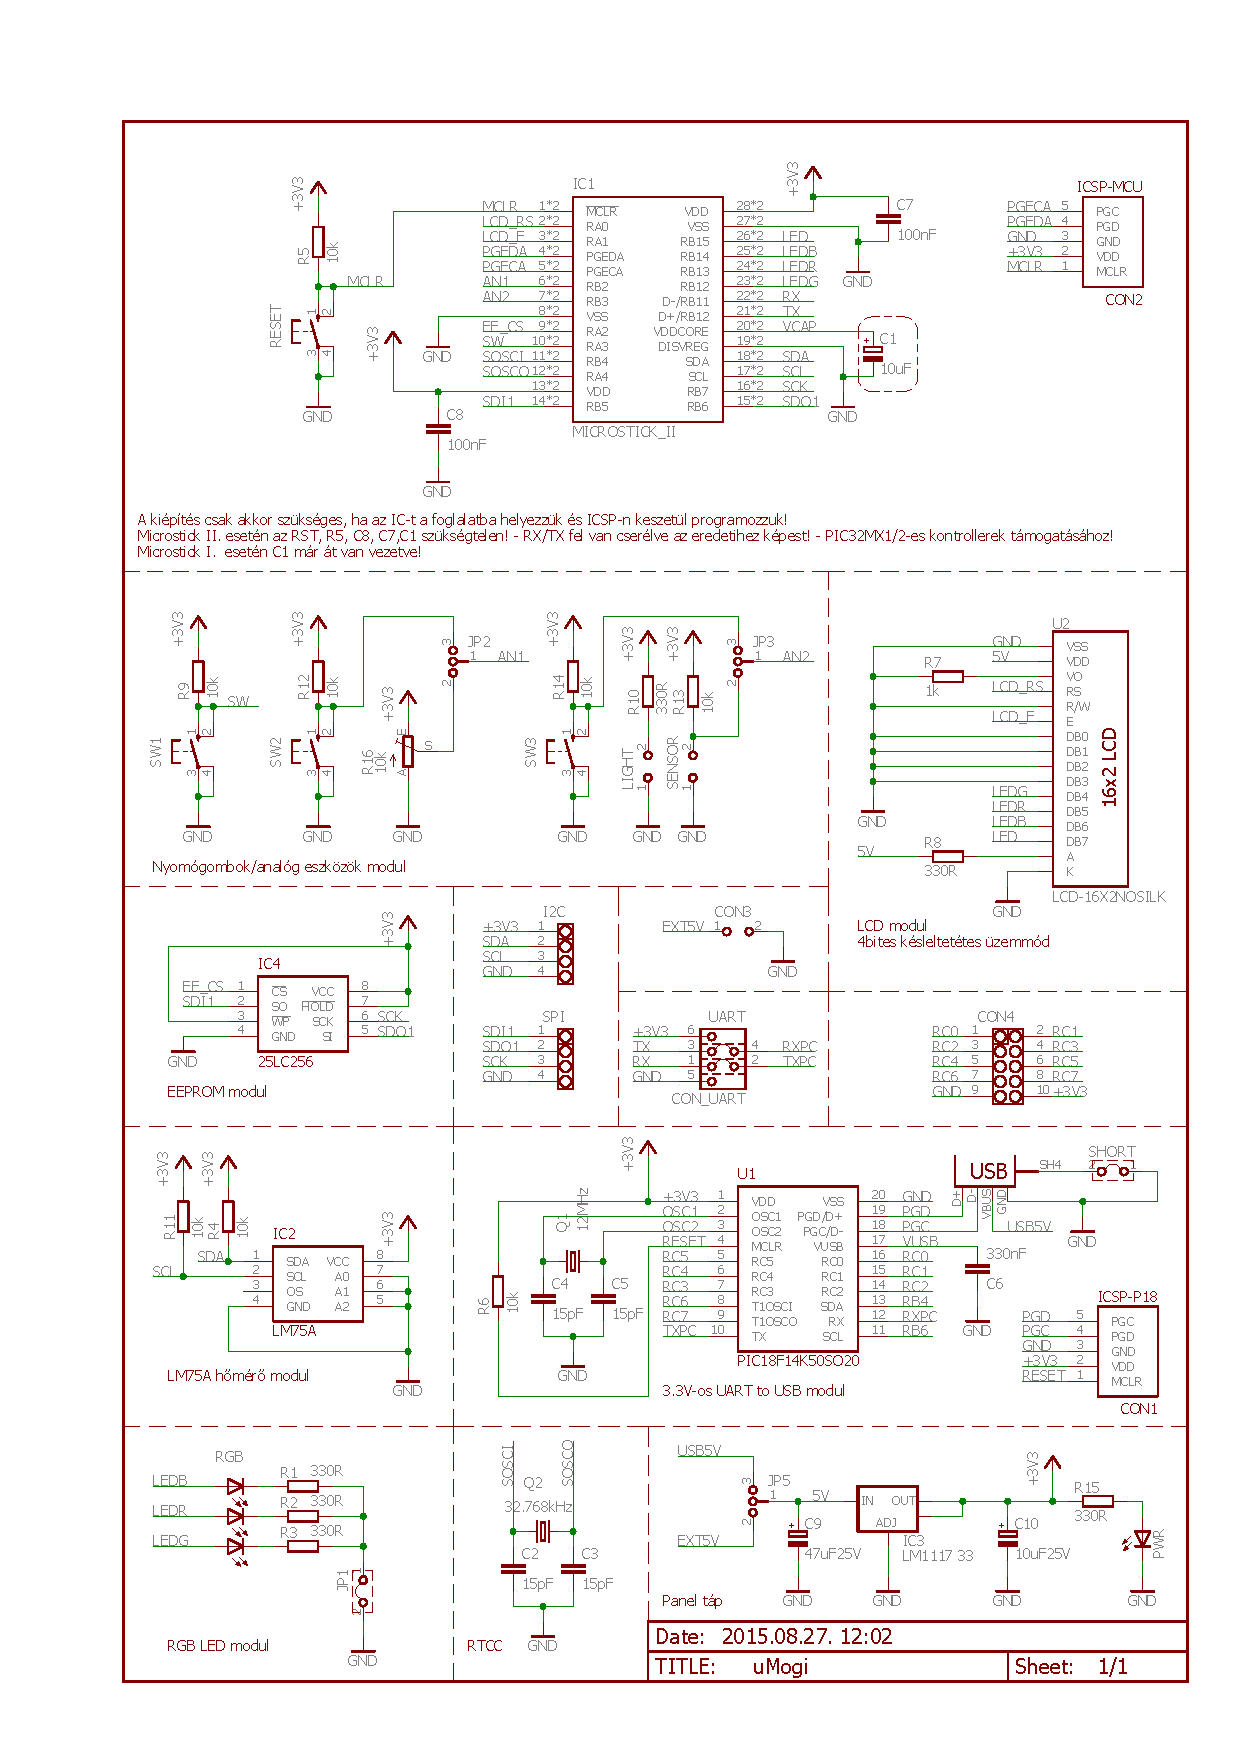
\includegraphics[width=0.9\textwidth, keepaspectratio]{figures/uMogi.pdf}
\caption{A uMogi kapcsolási rajza.} 
\end{figure}
          % Mellékletek - nem használt

\end{document}
